\section{Consommation de Soins et Biens Médicaux (14 points)}

Le tableau suivant donne la consommation de soins et biens médicaux (CSBM) en France de 2001 à 2008.

\begin{center}
	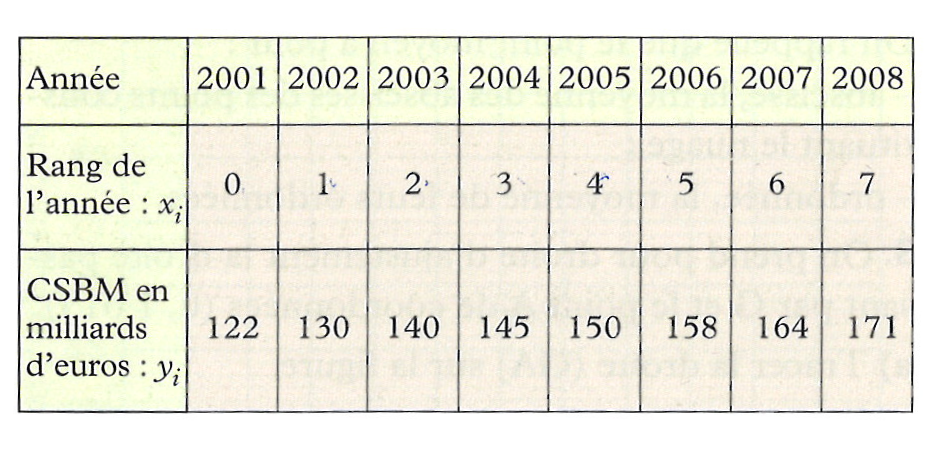
\includegraphics[scale=1.2]{csbm}
\end{center}

\begin{questions}
%	\question[1] Calculer le taux d'évolution de la CSBM entre 2001 et 2008. Arrondir à \num{0.01} \%.
	
	\question[1] Calculer le montant des dépenses de médicaments en 2008 sachant qu'elles représentaient \num{24.47}  \% de la CSBM. Arrondir au milliard.
	
	\question[2] Représenter par un nuage de points $M_i(x_i, y_i)$ la série statistique correspondant aux données du tableau. On utilisera un repère orthogonal du plan tel que :
	\begin{itemize}
		\item 1 cm représente une année sur l'axe des abscisses,
		
		\item 2 cm représentent 10 milliards d'euros sur l'axe des ordonnées (cet axe sera gradué de 100 à 200).
		
	\end{itemize}

	\question[4] 
		\begin{parts}
			\part[1] Calculer les coordonnées du point moyen G du nuage. Placer le point G sur le graphique.
			
			\part[2] Soit $\Delta$ la droite de coefficient directeur \num{6.7} passant par le point G ; déterminer une équation de la droite $\Delta$. Tracer la droite $\Delta$ sur le graphique.
			
			\part[1] Cette droite vous paraît-elle représenter un bon ajustement du nuage de points ? Pourquoi ?
		\end{parts}
	
		\question[2] On admet que l'ajustement réalisé par la droite $\delta$ est valable jusqu'en 2010. En laissant apparents les traits de construction, déterminer graphiquement :
			\begin{parts}
				\part[1]  Une estimation de la CSBM en 2010.
				\part[1] l'année au cours de laquelle la CSBM a dépassé 175 milliards d'euros.
			\end{parts}
		
		\question[2] Justifier par le calcul les résultats de la question précédente.
\end{questions}